\documentclass[tikz, border=1mm]{standalone}
\usetikzlibrary{arrows, shapes.gates.logic.US, calc}

\begin{document}
	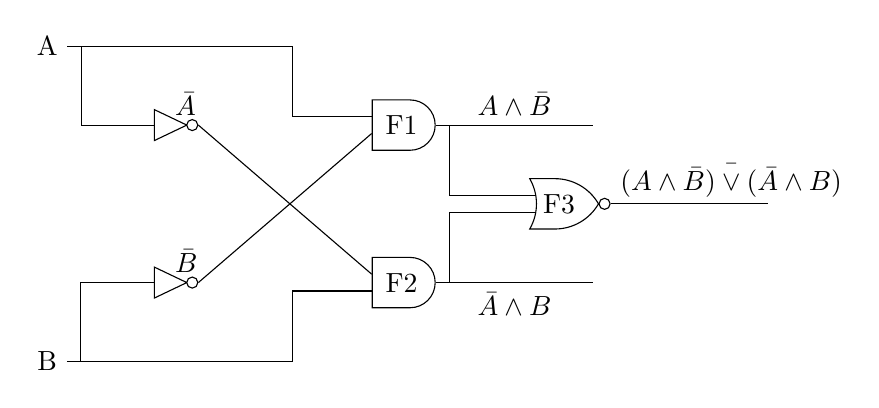
\begin{tikzpicture}
		\node (a) at (0,0) {A};
		\node (b) at (0,-4) {B};
		\node[not gate US, draw] at ($(a) + (1.5, -1)$) (nota) {};
		\node[not gate US, draw] at ($(b) + (1.5, 1)$) (notb) {};

		\node[and gate US, draw] at ($(nota) + (3, 0)$) (f1) {F1};
		\node[and gate US, draw] at ($(notb) + (3, 0)$) (f2) {F2};

		\draw ([xshift=5]a.east) |- (nota) node[above right]{$\bar{A}$}; 
		\draw (a.east) -| ([xshift=-1cm]f1.input 1) -- (f1.input 1);
		\draw ([xshift=5]b.east) |- (notb) node[above right]{$\bar{B}$};
		\draw (b.east) -| ([xshift=-1cm]f2.input 2) -- (f2.input 2) ;
		\draw (nota.output) -- (f2.input 1);
		\draw (notb.output) -- (f1.input 2);

		\node[nor gate US, draw] at ($(f1)!0.5!(f2) + (2,0)$) (f3) {F3};

		\draw (f2.output) -- ([xshift=5]f2.output) |- (f3.input 2);
		\draw (f2.output) -- ([xshift=2cm]f2.output) node[below, midway]{$\bar{A}\land{B}$};
		\draw (f1.output) -- ([xshift=5]f1.output) |- (f3.input 1);
		\draw (f1.output) -- ([xshift=2cm]f1.output) node[above, midway]{${A}\land\bar{B}$};
		\draw (f3.output) -- ([xshift=2cm]f3.output) node[above=3mm, right=-2cm] {$\bar{(A\land\bar{B})\lor(\bar{A}\land{B})}$};
	\end{tikzpicture}
\end{document}